\graphicspath{{../figures/}}

\newenvironment{Messtabelle}[1]
{\begin{minipage}{\linewidth} \centering  \begin{tabular}{#1} }
{\end{tabular} \vspace*{1em} \end{minipage}} 

\section{Turingmaschinen}

\begin{frame}{Grenzen endlicher Automaten}
	Automaten haben ja keinen Speicher außer ihren Zustand. \\
	\medskip
	\impl Ändern wir das: \\
	Nehmen wir nen Mealy-Automaten und ein unendlich langes Buchstabenband, das er lesen/beschreiben kann. \\
	\medskip
	Heraus kommt die...
\end{frame}

\subsection{Inhalt}
\begin{frame}{Turingmaschine}
	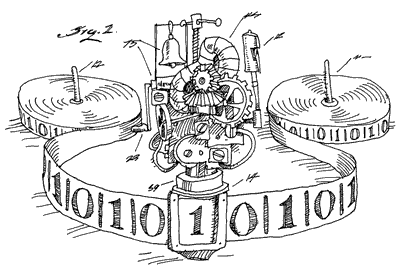
\includegraphics[scale=1]{turing/tmAufbau}
\end{frame}

% Kann ich erst Werbung für machen, nachdem ich ihn selbst gesehen habe, sonst wird's unglaubwürdig... :P
% Dann solltest du ihn unbedingt mal anschauen!
\thasse{
	\begin{frame}{Alan Turing}
		\centering
		\vspace{-25pt}
		
\includegraphics[scale=0.35]{turing/imitationGame}
	\end{frame}
}

%Das hier am Besten hinmalen mit Band und Schreiblesekopf und an der Tafel machen:
\begin{frame}{Eine einfache Turingmaschine}
	\begin{center}
		\begin{tikzpicture}[->,>=stealth,shorten >=1pt,auto,node distance=2.8cm,
		semithick,initial text={}]
		\tikzstyle{every state}=[]
		
		\node[initial,state] (A)                    {$a$};
		\node[state]         (M) [right of=A] 	    {$m$};
		
		\path 
		(A) edge [loop above] node {$\word 1\io\word 0R$} (A)
		edge [loop below]  node {$\word 0\io\word 1R$} (A)
		edge 					  node {$\word{2}\io\word{X}R$} (M)
		(M) edge [loop right] node {$\stackedtight{\word 0\io\word XR \\ \word 1\io\word XR \\ \word 2\io\word XR}$} (M)
		;
		\end{tikzpicture}
	\end{center} \pause
	Macht genau dasselbe wie der Automat von vorhin. \\ \pause
	\begin{tabular}{rl@{\ \?>\ }rl}
		Zustand vorher: & a &  nachher: & \hphantom{\word{100010}}a \\
		Band vorher: &\word{011101} &  nachher:&  \word{100010}$\9$\\
		\hline
		Zustand vorher: & a &  nachher: & \hphantom{\word{100010}}m \\
		Band vorher: &\word{011102} &  nachher:&  \word{10001X}$\9$\\
		\hline
		Zustand vorher: & a &  nachher: & \hphantom{\word{100010}}m \\
		Band vorher: &\word{012101} &  nachher:&  \word{10XXXX}$\9$\\
	\end{tabular}

\end{frame}



\begin{frame}{Turingmaschinen}
	Eine Turingmaschine besteht aus...
	\begin{itemize}[<+->]
		\item einem unendlichen Band mit einzelnen Zellen, in denen jeweils genau ein Symbol aus dem Bandalphabet steht
		\item einem Schreib-/Lesekopf, der auf genau einer Bandzelle steht
		\item einer Steuerungseinheit (Mealy-Automat), die sich in genau einem Zustand befindet
	\end{itemize}
\end{frame}

\begin{frame}{Funktionsweise der TM}
	In jedem Ausführungsschritt:
	\begin{itemize}[<+->]
		\item TM liest das Symbol, auf dem der Kopf steht
		\item Steuerung entscheidet über die Ausgabe, den Folgezustand und die Bewegung
		\item Ausgabe wird an der aktuellen Position auf das Band geschrieben
		\item Steuerung wechselt in den Folgezustand
		\item Kopf bewegt sich einen Schritt nach links (L) oder rechts (R) oder bleibt stehen (0)
	\end{itemize}
	\pause
	Die TM \textbf{hält}, wenn für einen Zustand und das gelesene Symbol keine Übergänge in der Steuerung definiert sind. \textbf{Eine TM muss nicht halten!} \\
	\impl Es können „Pfeile fehlen“!
\end{frame}

\begin{frame}{Eine einfache Turingmaschine v2}
	\begin{center}
		\begin{tikzpicture}[->,>=stealth,shorten >=1pt,auto,node distance=2.8cm,
		semithick,initial text={}]
		\tikzstyle{every state}=[]
		
		\node[initial,state] (A)                    {$a$};
		
		\path 
		(A) edge [loop above] node {$\word 1\io\word 0R$} (A)
		edge [loop below]  node {$\word 0\io\word 1R$} (A)
		;
		\end{tikzpicture}
	\end{center} \pause
	Pfeil für Eingabe \word 2 fehlt jetzt! \pause \impl TM hört dann einfach auf! \\ \pause
	\begin{tabular}{rl@{\ \?>\ }rl}
		Zustand vorher: & a &  nachher: & \hphantom{\word{100010}}a \\
		Band vorher: &\word{011101} &  nachher:&  \word{100010}$\9$\\
		\hline
		Zustand vorher: & a &  nachher: & \hphantom{\word{10001}}a \\
		Band vorher: &\word{011102} &  nachher:&  \word{100012}\\
		\hline
		Zustand vorher: & a &  nachher: & \hphantom{\word{10}}a \\
		Band vorher: &\word{012101} &  nachher:&  \word{102101}\\
	\end{tabular}
	
\end{frame}

\begin{frame}{Eine einfache Turingmaschine, Rage-Mode!}
	\begin{center}
		\begin{tikzpicture}[->,>=stealth,shorten >=1pt,auto,node distance=2.8cm,
		semithick,initial text={}]
		\tikzstyle{every state}=[]
		
		\node[initial,state] (A)                    {$a$};
		\node[state]         (M) [right of=A] 	    {$m_1$};
		\node[state]         (M2) [right of=M] 	    {$m_2$};
		
		\path 
		(A) edge [loop above] node {$\stackedtight{\word 1\io\word 0R \\ \word 0\io\word 1R}$} (A)
		edge 					  node {$\word{2}\io\word{2}R$} (M)
		(M) edge [loop above] node {$\stackedtight{\word 0\io\word 0R \\ \word 1\io\word 1R \\ \word 2\io\word 2R}$} (M)
		edge 					  node {$\9\io\9L$} (M2)
		(M2) edge [loop right] node {$\stackedtight{\word 0\io\9L \\ \word 1\io\9L \\ \word 2\io\9L}$} (M2)
		;
		\end{tikzpicture}
	\end{center} \pause
	\impl Löscht das komplette Eingabewort, wenn sie ne \word 2 in die Finger kriegt! \smiley \\ \pause
	\begin{tabular}{rl@{\ \?>\ }rl}
		Zustand vorher: & a &  nachher: & \hphantom{\word{100010}}a \\
		Band vorher: &\word{011101} &  nachher:&  \word{100010}$\9$\\
		\hline
		Zustand vorher: & a &  nachher: & $m_2$\\
		Band vorher: &\word{011102} &  nachher:&  $\9\9\9\9\9\9$\\
		\hline
		Zustand vorher: & a &  nachher: & $m_2$ \\
		Band vorher: &\word{012101} &  nachher:& $\9\9\9\9\9\9$\\
	\end{tabular}
\end{frame}

\begin{frame}{Ein-/Ausgabe}
	\begin{block}{Eingabe}
		Am Anfang steht das Eingabewort umgeben von Blanksymbolen auf dem Band, der Kopf steht auf dem ersten Zeichen des Eingabeworts.
	\end{block}
	\pause
	
	\begin{block}{Ausgabe}
		Zwei Möglichkeiten:
		\begin{itemize}[<+->]
			\item Berechnung von Funktionen: Ausgabewort steht am Ende auf dem Band \\
			\impl „normale“ TMen
			\item Erkennen von Sprachen: Halten in akzeptierendem Zustand (Doppelkringel)\\
			\impl Turingmaschinen-\textbf{Akzeptor} \\
				  Wir bezeichnen dann wieder mit $L(T)$ die akzeptierte Sprache \\
				  (Was aufm Band steht, ist dann bloß Nebenrechnung.)
		\end{itemize}
	\end{block}
\end{frame}

\begin{frame}{Konfigurationen}
	Den „Gesamtzustand“ einer Turingmaschine (also akt. Zustand, Bandinhalt und Schreibkopf-Position) nennen wir \textbf{Konfiguration}. \\ \pause
	\medskip
	In GBI schreiben wir dafür das aktuelle Wort auf dem Band und über das Zeichen, auf dem der Kopf grade steht, den Zustand. \\
	Beispiel: \\
	\bigskip
	\mbox{}\hphantom{\word{100}$\9$.\!}z \\
	\mbox{\word{100}$\9$\word{101}}
	
	\pause \bigskip
	(Formalkram dazu: \impl VL!)
\end{frame}

\mycomment{ %TODO Fix. Oder gleich an der Tafel machen erkläutern, wie das mit Konfigurationen geht. IMHO besser.
	\begin{frame}{Beispiel}
		\vspace{-30pt}
		\begin{center}
			
			\begin{tikzpicture}[shorten >=1pt,initial text=,node distance=2cm,auto,->,>=stealth,baseline=(B.base)]
			% \node[state,initial]  (S)                       {$S$};
			\node[state,initial]  (A)          {$A$};
			% \node (nix) [right of=A] {};
			\node[state]          (B) [above right of=A] {$B$};
			\node[state]          (C) [right of=B] {$C$};
			\node[state]          (E) [below right of=A] {$E$};
			\node[state]          (D) [right of=E] {$D$};
			\path[->]
			% (S) edge              node  {$\9\io\9R$} (A)
			(A) edge              node  {$\word 1\io\word XR$} (B)
			(B) edge [loop above] node  {$\word 1\io\word 1R$} ()
			edge              node  {$\9\io\9R$} (C)
			(C) edge [loop above] node  {$\word 1\io\word 1R$} ()
			edge              node  {$\9\io\word 1L$} (D)
			(D) edge [loop below] node  {$\word 1\io\word 1L$} ()
			edge              node  {$\9\io\9L$} (E)
			(E) edge [loop below] node  {$\word 1\io\word 1L$} ()
			edge              node  {$\word X\io\word 1R$} (A)
			% (B) edge              node        {$\9\io\9R$} (B)
			% edge [loop right] node        {$\#1\io\#1R$} ()
			% (B) edge [loop right] node {$\9\io\#1L$} ()
			% edge  node [pos=0.3]       {$\#1\io\#1L$} (A)
			;
			\end{tikzpicture}
			\bigskip
			
			\begin{tabular}{c|c|c|c|c|c}
				%	& A & B & C & D & E \\ \hline
				%	$\square $ & & C,$\square$,R & D, $\word 1$, L & E,$\square$, L & \\ \hline
				%	$\word 1$ & B,$X$, R & B,$\word 1$, R & C,$1$, R & D,$\word 1$, L & E,$\word 1$, L \\ \hline
				%	$X$ & & & & & A,$\word 1$,R \\
			\end{tabular}
		\end{center}
	\end{frame}
	
	% DIESES BEISPIEL IST FEHLERHAFT!
	\begin{frame}[t]{Beispiel}
		\only<1|handout:1>{Eingabe: $11$}
		\bigskip
		\begin{itemize}
			\only<1-3|handout:1>{\item[1] \begin{Messtabelle}{ccccccc} & A & & & & & \\ & $\downarrow$ &&&&& \\ 
					$\square$ & 1 & 1 & $\square$ & $\square$ & $\square$ & $\square$ \end{Messtabelle} }
			\only<2-4|handout:1>{\item[2] \begin{Messtabelle}{ccccccc} &  & B & & & & \\ & &$\downarrow$ &&&& \\ 
					$\square$ & X & 1 & $\square$ & $\square$ & $\square$ & $\square$ \end{Messtabelle} }
			\only<3-5|handout:1>{\item[3] \begin{Messtabelle}{ccccccc} &  & & & C& &  \\ &  &&& $\downarrow$ & &\\ 
					$\square$ & X & 1 & $\square$ & $\square$ & $\square$ & $\square$ \end{Messtabelle} }
			\only<4-6|handout:2>{\item[4] \begin{Messtabelle}{ccccccc} &  & & D & & &  \\ &  && $\downarrow$ &&& \\ 
					$\square$ & X & 1 & $\square$ & 1 & $\square$  & $\square$ \end{Messtabelle} }
			\only<5-7|handout:2>{\item[5]  \begin{Messtabelle}{ccccccc} &  & E &  & & &  \\ &  & $\downarrow$ &&&& \\ 
					$\square$ & X & 1 & $\square$ & 1 & $\square$  & $\square$ \end{Messtabelle} }
			\only<6-8|handout:2>{ \item[6] \begin{Messtabelle}{ccccccc} &  &   A && & &  \\ &  &  $\downarrow$ &&&& \\ 
					$\square$ & 1 & 1 & $\square$ & 1 & $\square$  & $\square$ \end{Messtabelle} }
			\only<7-9|handout:3>{\item[7] \begin{Messtabelle}{ccccccc} &  &    & B & & &  \\ &  &&  $\downarrow$ &&& \\ 
					$\square$ & 1 & X & $\square$ & 1 & $\square$  & $\square$ \end{Messtabelle} }
			\only<8-10|handout:3>{\item[8] \begin{Messtabelle}{ccccccc} &  &    &  & & C &  \\ &  && && $\downarrow$ & \\ 
					$\square$ & 1 & X & $\square$ & 1 & $\square$  & $\square$ \end{Messtabelle} }
			\only<9-11|handout:3>{\item[9] \begin{Messtabelle}{ccccccc} &  &    &  &  D& &  \\ &  && & $\downarrow$ && \\ 
					$\square$ & 1 & X & $\square$ & 1 & 1  & $\square$ \end{Messtabelle} }
			\only<10-12|handout:4>{\item[10] \begin{Messtabelle}{ccccccc} &  &   E &  &  & &  \\ &   & $\downarrow$ && &&\\ 
					$\square$ & 1 & X & $\square$ & 1 & 1  & $\square$ \end{Messtabelle} }
			\only<11-12|handout:4>{\item[11] \begin{Messtabelle}{ccccccc} &  &    & A &  & &  \\ &   && $\downarrow$ && &\\ 
					$\square$ & 1 & 1 & $\square$ & 1 & 1  & $\square$ \end{Messtabelle} }
		\end{itemize}
		\only<12|handout:4>{ Also allgemein : Eingabe von $1^k$ wird zu $\square \, 1^k \, \square \, 1^k \, \square $} 
	\end{frame}
}


\begin{frame}{Turingmaschine}
	\begin{Definition}
		Eine Turingmaschine $T$ ist definiert als $$ T = (Z, z_0 , X, f,g, m)$$
		\begin{itemize}[<+->]
			\item $Z \quad$ Zustandsmenge 
			\item $z_0\in Z \quad$ Startzustand
			\item $X \quad$ Bandalphabet mit $\square \in X$
			\item $f:Z\times X \dashrightarrow Z \quad$ Übergangsfunktion
			\item $g:Z\times X\dashrightarrow X \quad$ Ausgabefunktion  \quad (\textbf{genau ein Zeichen} als Ausgabe!)
			\item $m:Z\times X \dashrightarrow \{\text{L},\text{0},\text{R}\} \quad$ Bewegungsfunktion
		\end{itemize}
		\pause
		Alle Funktionen können auch nur partiell definiert ($\dashrightarrow$) sein. \\
		(Heißt: Sie sind nicht linkstotal $=$ Es fehlen Pfeile.)
	\end{Definition}
\end{frame}

\begin{frame}{Beispiel: Formale Definition}
	\begin{center}
		\begin{tikzpicture}[->,>=stealth,shorten >=1pt,auto,node distance=2.8cm,
		semithick,initial text={}]
		\tikzstyle{every state}=[]
		
		\node[initial,state] (A)                    {$a$};
		\node[state]         (M) [right of=A] 	    {$m_1$};
		\node[state]         (M2) [right of=M] 	    {$m_2$};
		
		\path 
		(A) edge [loop above] node {$\stackedtight{\word 1\io\word 0R \\ \word 0\io\word 1R}$} (A)
		edge 					  node {$\word{2}\io\word{2}R$} (M)
		(M) edge [loop above] node {$\stackedtight{\word 0\io\word 0R \\ \word 1\io\word 1R \\ \word 2\io\word 2R}$} (M)
		edge 					  node {$\9\io\9L$} (M2)
		(M2) edge [loop right] node {$\stackedtight{\word 0\io\9L \\ \word 1\io\9L \\ \word 2\io\9L}$} (M2)
		;
		\end{tikzpicture}
	\end{center}
	\begin{align*}
		\text{Bandalphabet } X &= \set{\word 0, \word 1, \word 2, \9} \\
		f(a,\word 1) &= a	\\
		f(a, \9) &\text{ ist nicht definiert.} \\ 
		g(a, \word 1) &= \word 0 \\
		g(a, \9) &\text{ ist nicht definiert.} \\ 
		m(m_1, \9) &= L \\
		m(m_2, \9) & \text{ ist nicht definiert.}
	\end{align*}
\end{frame}

\begin{frame}{Aufgabe}
	Was macht die folgende Turingmaschine für Eingaben aus $\{\word 0, \word 1\}^*$?
	
	%\smallskip
	%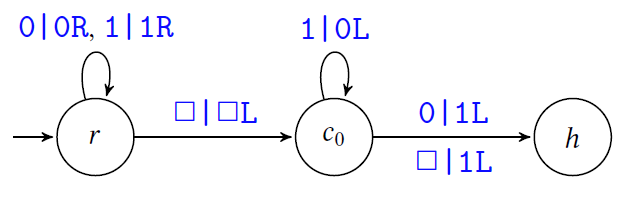
\includegraphics[scale=0.65]{turing/addBin1}
	\begin{center}
		\begin{tikzpicture}[->,>=stealth,shorten >=1pt,auto,node distance=2.8cm,
		semithick,initial text={}]
		\tikzstyle{every state}=[]
		
		\node[initial,state] (R)                    {$r$};
		\node[state]         (C) [right of=R] 	    {$c_0$};
		\node[state]         (H) [right of=C] 	    {$h$};
		
		\path 
		(R) edge [loop above] node {$\word 0\io\word 0R, \word 1\io\word1R$} (R)
		edge 					  node {$\9\io\9L$} (C)
		(C) edge [loop above] node {$\word 1\io\word 0L$} (C)
		edge 					  node {$\stackedtight{\word 0\io\word 1L, \\ \9\io\word 1L }$} (H)
		;
		\end{tikzpicture}
	\end{center}
	
	\smallskip
	\visible<2|handout:2>{
		Inkrementieren der dargestellten Zahl um $1$.
	}
\end{frame}

\begin{frame}{Aufgabe}
	Entwerft eine Turingmaschine, die für eine Eingabe $w \in \{\word 0, \word 1\}^*$ $$\fRepr_2(\fNum_2(w) - 1)$$ berechnet. Ihr dürft davon ausgehen, dass $\fNum_2(w) > 0$ gilt.\\
	\visible<2-|handout:2->{
		\begin{center}
			\begin{tikzpicture}[->,>=stealth,shorten >=1pt,auto,node distance=2.8cm,
			semithick,initial text={}]
			\tikzstyle{every state}=[]
			
			\node[initial,state] (R)                    {$r$};
			\node[state]         (C) [right of=R] 	    {$c_0$};
			\node[state]         (H) [right of=C] 	    {$h$};
			
			\visible<4-|handout:3->{
				\node[state]         (Z) [below=1cm of H] 	    {$z$};
			}
			\visible<6-|handout:4->{
				\node[state]         (L) [below=1cm of C] 	    {$\ell$};
			}
			
			\path 
			(R) edge [loop above] node {$\word 0\io\word 0R, \word 1\io\word1R$} (R)
			edge 					  node {$\9\io\9L$} (C)
			(C) edge [loop above] node {$\word 0\io\word 1L$} (C)
			edge 					  node {$\word 1\io\word 0L$} (H);
			
			\visible<4-|handout:3->{
				\path
				(H) edge [loop above] node {$\word 0\io\word 0L, \word 1\io\word1L$} (H)
				edge [left]				  node {$\9\io\9R$} (Z)
				(Z)  edge [loop right] node {$\word 0\io\9R$} (Z);
			}
			
			\visible<6-|handout:4->{
				\path
				(Z)  edge 				 node[below] {$\9\io\word 0L$} (L);
			}
			\end{tikzpicture}
		\end{center}
	}
	\visible<3-|handout:3->{\§{\textbf{Achtung}:} Was passiert mit führenden Nullen?} \\ 
	\visible<5-|handout:4->{\. Was, wenn es nur eine \word 0 gibt?} \\	
\end{frame}

\begin{frame}{Aufgabe}
	Wie würde man eine (einfache, nicht effiziente) TM zum Addieren von zwei Zahlen in Binärdarstellung aufbauen? \\ \pause
	\smallskip
	\impl Inkrementiere erste Zahl, dekrementiere zweite Zahl. Wiederhole, bis zweite Zahl $= 0$.
\end{frame}

\def\bword#1{\texttt{#1}}
\begin{frame}[t]{TM-Akzeptoren}
	\only<all:1>{
		Erinnerung: Inkrementieren um eins 
		\begin{center}
			\begin{tikzpicture}[->,>=stealth,shorten >=1pt,auto,node distance=2.8cm,
				semithick,initial text={}]
				\tikzstyle{every state}=[]
				
				\node[initial,state] (R)                    {$r$};
				\node[state]         (C) [right of=R] 	    {$c_0$};
				\node[state]         (H) [right of=C] 	    {$h$};
				
				\node[state,accepting,white]         (A) [below of=H] 	    {\phantom{$a_1$}};
				\node[state,white]         (B) [below of=C] 	    {\phantom{$a_2$}};
				
				\path 
				(R) edge [loop above] node {$\word 0\io\word 0R, \word 1\io\word 1R$} (R)
				edge 					  node {$\9\io\9L$} (C)
				(C) edge [loop above] node {$\word 1\io\word 0L$} (C)
				edge 					  node {$\stackedtight{\word 0\io\word 1L \\ \9\io\word 1L}$} (H)
				
				(H) edge [loop above,white] node {\phantom{$\word 0\io\word 0L, \word 1\io\word 1L$}} (H)
				(A)  edge [white]				 node[below] {\phantom{$\word 0\io\word 0L$}} (B)
				;
			\end{tikzpicture}
		\end{center}
	\mbox{}\vphantom{Welche Sprache....} \\
	}
	\only<all:2->{
		\?> TM-Akzeptor: 
		\begin{center}
			\begin{tikzpicture}[->,>=stealth,shorten >=1pt,auto,node distance=2.8cm,
				semithick,initial text={},every initial by arrow/.style={gray}]
				\tikzstyle{every state}=[]
				
				\node[initial,state,gray] (R)                    {$r$};
				\node[state,gray]         (C) [right of=R] 	    {$c_0$};
				\node[state]         (H) [right of=C] 	    {$h$};
				
				\node[state,accepting]         (A) [below of=H] 	    {$a_1$};
				\node[state]         (B) [below of=C] 	    {$a_2$};
				
				\path 
				(R) edge [loop above,gray] node {$\bword 0\io\bword 0R, \bword 1\io\bword 1R$} (R)
				edge [gray] 					  node {$\9\io\9L$} (C)
				(C) edge [loop above,gray] node {$\bword 1\io\bword 0L$} (C)
				edge [gray] 					  node {$\stackedtight{\bword 0\io\bword 1L \\ \9\io\bword 1L}$} (H)
				
				(H) edge [loop above] node {$\word 0\io\word 0L, \word 1\io\word 1L$} (H)
				edge [left]				  node {$\9\io\9R$} (A)
				(A)  edge [loop above left] node[left] {$\word 1\io\word 1R$} (A)
				(A)  edge 				 node[below] {$\word 0\io\word 0R$} (B)
				;
			\end{tikzpicture}
		\end{center}
		Welche Sprache akzeptiert diese TM? \\
	}
	\medskip
	\visible<3-|handout:2->{$\impl L(T) = \set{w \in \set{\word 0,\word 1}^* \Mid \fRepr_2(\fNum_2(w) + 1) \in \set{\word 1}^*}$}
\end{frame}

\begin{frame}{Turing-Maschinen vs. Supercomputer}
	Eine TM kann \textbf{genauso viel} berechnen wie euer Handy oder ein Supercomputer von Intel. {\small (Bloß halt etwas langsamer und umständlicher!)} \\
	\medskip
	Es gibt kein „mächtigeres“ Maschinenmodell als Turingmaschinen. \\
	\only<beamer:0>{
		\medskip 
		\begin{center}
			\impl Was eine Turingmaschine nicht berechnen \\ kann, kann keiner berechnen. \smiley \\ \#Prädikatenlogik-Blatt 2017/18
		\end{center}
	}
\end{frame}

\mycomment{ % Formalkram ist bähhh...
	% Ja, aber eigentlich wichtig. Aber dieses Jahr keine Zeit.
	\begin{frame}{Konfiguration}
		\begin{Definition}
			Als \textbf{Konfiguration} $ c =(z,b,p)$ bezeichnen wir den Zustand einer Turing-Maschine zu einem Zeitpunkt. Dabei ist 
			\begin{itemize}
				\item $z\in Z$ der Zustand
				\item $b: \Z\to X$ die Bandbeschriftung
				\item $p\in \Z$ die Position des Zeigers.
			\end{itemize}
		\end{Definition}
	\end{frame}
	
	\begin{frame}{Berechnungsschritte}
		\begin{Definition}
			In einem Berechnungsschritt geht eine TM aus einer Konfiguration $c$ 
			in die Konfiguration $$\Delta_1(c) := c' = (z',b',p')$$ über, wobei gilt:
			\begin{itemize}[<+->]
				\item $z' = f(z,b(p))$
				\item $\forall i\in \Z: b'(i) =
				\begin{cases}
				b(i) & \text{ falls } i\not=p \\
				g(z,b(p)) & \text{ falls } i=p
				\end{cases}$
				\item $p' = p + m(z,b(p))$
			\end{itemize}
			\bigskip
			
			\pause
			Wenn $\Delta_1(c)$ nicht definiert ist, bezeichnet man $c$ als \textbf{Endkonfiguration} und die TM \textbf{hält}.
		\end{Definition}
	\end{frame}
	
	\begin{frame}{Berechnungen}
		\begin{Definition}
			Eine Berechnung ist eine Folge von Konfigurationen $(c_0, c_1, ..., c_t)$ bei der gilt $$c_{i+1} = \Delta_1(c_i)$$ \pause
			Es gibt endliche, haltende (endet in einer Endkonfiguration) und unendliche Berechnungen.
			\bigskip
			
			\pause
			Induktiv definiert man $\Delta_t(c) , t\in\N_0$ als die Konfiguration, welche nach $t$ Berechnungsschritten erreicht werden kann und $\Delta_*(c)$ als Endkonfiguration, die von $c$ aus erreicht wird (falls die Berechnung endet).
		\end{Definition}
	\end{frame}
}








\begin{frame}{Entscheidbarkeit}
	\begin{Definition}
		Eine Sprache $L$ ist eine   
		\begin{itemize}[<+->]
			\item \textbf{aufzählbare Sprache}, wenn es eine Turingmaschine gibt, die $L$ akzeptiert.
			\item \textbf{entscheidbare Sprache}, wenn es eine Turingmaschine gibt, die $L$ akzeptiert und \emph{für jede Eingabe} hält.
		\end{itemize}
	\end{Definition} \pause
	
	Bei aufzählbaren Sprachen ist nicht definiert, wie sich die TM für Wörter $ w \notin L$ verhält. Sie kann diese ablehnen oder nicht halten. Ob eine TM für eine Eingabe nicht hält, können wir \enquote{von außen} nicht einfach feststellen.
\end{frame}
